% This is samplepaper.tex, a sample chapter demonstrating the
% LLNCS macro package for Springer Computer Science proceedings;
% Version 2.20 of 2017/10/04
%
\documentclass[runningheads]{llncs}
%
\usepackage{graphicx,subfig}
\usepackage{amstext,amsmath,amssymb,bm,bbm,mathtools}

\newtheorem{ddef}{Definition}
\DeclareMathOperator*{\argmin}{arg\,min}
\DeclarePairedDelimiter\norm{\lVert}{\rVert}%
\DeclarePairedDelimiter\abs{\lvert}{\rvert}%

% Used for displaying a sample figure. If possible, figure files should
% be included in EPS format.
%
% If you use the hyperref package, please uncomment the following line
% to display URLs in blue roman font according to Springer's eBook style:
% \renewcommand\UrlFont{\color{blue}\rmfamily}

\begin{document}
%
\title{Digital Curvature Evolution Model for Image Segmentation\thanks{This  work has  been  partly  funded by CoMeDiC ANR-15-CE40-0006 research grant.}}

\author{Daniel Antunes\inst{1}
Jacques-Olivier Lachaud\inst{1}
Hugues Talbot\inst{2}}
%
\authorrunning{D. Antunes et al.}
% First names are abbreviated in the running head.
% If there are more than two authors, 'et al.' is used.
%
\institute{Laboratoire de Mathematiques (LAMA), Universite Savoie Mont Blanc, Chamb\'ery, France
\email{daniel.martins-antunes, jacques-olivier.lachaud@univ-savoie.fr} \and
CentraleSupelec Universit\'e Paris-Saclay\\
\email{hugues.talbot@centralesupelec.fr}}
%
\maketitle              % typeset the header of the contribution
%
\begin{abstract}
  Recent works have indicated the potential of using curvature as a
  regularizer in image segmentation, in particular for the class of
  thin and elongated objects. These are ubiquitous in bio-medical
  imaging (e.g. vascular networks), in which length regularization can
  sometime performs badly, as well as in texture
  identification. Curvature is a second-order differential measure,
  and so its estimators are sensitive to noise. The straightforward
  extentions to Total Variation are not convex, making it a challenge
  to optimize.  State-of-art techniques make use of a coarse
  approximation of curvature that limit practical applications.

  We argue that curvature must be computed
  using a multigrid convergent estimator, instead, which we propose
  in this article. We illlustrate the use of the model as a post-processing step in a
  segmentation framework.
 
\keywords{Multigrid convergence  \and Digital estimator \and Curvature \and Shape Optimization \and Image Segmentation.}
\end{abstract}
%
%
%
\setcounter{footnote}{0}
\section{Introduction}

Geometric quantities are particularly useful as regularizers, especially when object geometry is known a priori. Length penalization is a general purpose regularizer and the literature is vast on models that make use of it \cite{casseles97,appleton05}. However, this regularizer is not suitable for the segmentation of thin and elongated objects, as it tends to return disconnected solutions. Such drawback can be overcomed by injecting curvature regularization \cite{zehiry10}.
				
One of the first successful uses of curvature in image processing is the inpainting algorithm described in \cite{masnou98}. The author evaluates the elastica energy along the level lines of a simply-connected image to reconstruct its occluded parts. The level lines property of non-intersection allows the construction of an efficient dynamic programming algorithm. Nonetheless, it is still a challenging task to inject curvature in the context of image segmentation. 

The state-of-art methods are difficult to optimize and  not scalable \cite{zehiry10,schoenemann09,nieuwenhuis14}. In order to achieve reasonable running times, such approaches make use of a coarse and not convergent approximation of curvature, which has an important impact in the results. Recently, multigrid convergent estimators for curvature have been proposed \cite{schindele17,coeurjolly13,roussillon11}, motivating us to search for models in which they can be applied.

In this work, we investigate the use of a more suitable curvature estimator with multigrid convergent property and its application as boundary regularizer. Our method reduces the elastica energy of the contour and we illustrate its behaviour by evaluating several digital flows. Finally, we present an application of the model as a post-processing step on a segmentation framework. The code is made available at github\footnote{https://www.github.com/danoan/DGCI19}.

\textit{Outline}. Section two reviews the concept of multigrid convergence and highlights its importance on the definition of digital estimators. Next, we describe two convergent estimators used in this paper, one for tangent and the other for curvature. They are used on the optimization model and in the definition of the digital elastica. Section three describes the proposed curvature evolution model along with several illustrations of digital flows. Section four explains how to use the evolution model as a post-processing step in a image segmentation framework. Finally, sections five and six discuss the results and point directions for future work.




\section{Multigrid Convergent Estimators}



A digital image is the result of some quantization process (e.g. Gauss digitization) over an object $X$ residing in some continuous space of dimension $d$. Such process is parameterized by a scale parameter $h>0$ and generates the object $D_h(X) \subset h \cdot \mathbb{Z}^d$, the digitization of $X$ in a grid space of size $h$. 

Given a object $X$ and its digitization $D_h(X)$, a digital estimator $\hat{u}$ for some geometric quantity $u$ is intended to compute $u(X)$ by using only the digitization. This problem is not well posed, as the same digital object could be the digitization of infinitely others objects very different from $X$. Therefore, a characterization of what is a good estimator is necessary.

Let $u$ be some geometric quantity of $X$ (e.g. tangent, curvature). We wish to devise a digital estimator $\hat{u}$ for $u$. It is reasonable to state that $\hat{u}$ is a good estimator if $\hat{u}(D_h(X))$ converges to $u(X)$ as we refine our grid. For example, counting pixels is a convergent estimator for area; but counting boundary pixels is not a convergent estimator for perimeter. Multigrid convergence is the mathematical tool that makes this definition precise.


	
	\begin{ddef}[Multigrid convergence for local geometric quantites]
		A local discrete geometric estimator $\hat{u}$ of some geometric quantity $u$ is multigrid convergent for the family $\mathbb{X}$ if and only if, for any $X \in \mathbb{X}$, there exists a grid step $h_X>0$ such that the estimate $\hat{u}(D_h(X),\hat{x},h)$ is defined for all $\hat{x} \in \partial_hX$ with $ 0 < h < h_X$, and for any $x \in \partial X$,
		
		\begin{equation}
			\forall \hat{x} \in  \partial_hX \text{ with } \norm{ \hat{x} - x }_{\infty} \leq h, \norm{ \hat{u}(D_h(X),\hat{x},h) - u(X,x)} \leq \tau_{X,x}(h),			
		\end{equation}
		
		where $\tau_{X,x}:\mathbb{R}^{+}\setminus\{0\} \rightarrow \mathbb{R}^{+}$ has null limit at $0$. This function defines the speed of convergence of $\hat{u}$ towards $u$ at point $x$ of $X$. The convergence is uniform for $X$ when every $\tau_{X,x}$ is bounded from above by a function $\tau_X$ independent of $x \in \partial X$ with null limit at $0$.
	\end{ddef}
	
	
	For a global geometric quantity (e.g. perimeter, area, volume), the definition remains the same, except that the mapping between $\partial X$ and $\partial_h X$ is no longer necessary.
	
	
	Multigrid convergent estimators give us a quality certificate and should be preferred over non-multigrid convergent ones. In the next section we describe two estimators that will be important for our purpose.
	


\subsection{Tangent and Perimeter Estimators}

The literature presents several perimeter estimators which are multigrid convergent (see \cite{coeurjolly04,coeurjolly12} for a review), but in order to define the digital elastica we need a local estimation of length and we wish that integration over these local length elements gives a multigrid convergent estimator for the perimeter. 

\begin{ddef}[Elementary Length]
	Let a digital curve $C$ to be represented as a sequence of grid vertices in a grid cell representation of digital objects. Further, let $\hat{\theta}$ to be a multigrid convergent estimator for tangent. The elementary length $\hat{s}(e)$ at some grid edge $e\in C$ is defined as
	
	\begin{align*}
		\hat{s}(e) = \hat{\theta(l)} \cdot or(e),
	\end{align*}
	where $or(e)$ denotes the grid edge orientation.
\end{ddef}

	In \cite{lachaud06}, Lachaud proves that the integration of the elementary length along the digital curve is a multigrid convergent estimator for perimeter if one uses the $\lambda$-MST \cite{lachaud07} tangent estimator.



%We represent a curve as a sequence of pointels (zero dimensional elements of the digital grid. Its respective higher dimensional counterparts are called linels and pixels). Sequence indexes are recovered by function $i_C(\cdot)$. The curve segment $C_{p,q}$ between pointels $p,q$ is a digital straight segment (DSS) if $C_{p,q}$ is a standard line.
%
%
%\begin{ddef}[Standard line] 
%The set of points
%$(x, y)$ of the digital plane verifying $\mu \leq ax -by \leq \abs{a} + \abs{b}$ , with $a,b$ and $\mu$
%integer numbers, is called the standard line
%with slope $a/b$ and shift $\mu$.
%\end{ddef}
%
%The $\lambda$-MST estimates the tangent of some curve $C$ at some pointel $p$ as a ponderated sum over the set of maximal digital straight segments of $C$ containing $p$.
%
%
%
%The curve $C$ can be covered by its set of maximal DSS $\mathcal{S}$. Hence, every pointel belongs to at least one maximal DSS. In fact, a pointel $p$ can be present in two or more elements of $\mathcal{S}$. We denote the pencil of $p$ by $\mathcal{P}(p) \subset \mathcal{S}$ as the set of maximal DSS which passes through $p$. We are now ready to characterize the eccentricity between a pointel $p$ and its pencil elements $M \in \mathcal{P}(p)$.
%
%\begin{align*}
%	e_p(M) = \frac{\abs{i_M(p) - i_M(q)} }{\abs{M}}. 
%\end{align*}
%
%The eccentricity is used to define the weight function $\lambda:[0,1]\rightarrow \mathbb{R}^+$. A good choice would be bell-shaped functions as the $C^2$ function $64(-x^6 + 3x^5 - 3x^4 + x^3)$ or the $C^{\infty}$ function $exp(4 - \frac{1}{x} - \frac{1}{1-x}).$ as noted by \cite{lachaud07}.
%
%\begin{ddef}[$\lambda$-MST] 
%The $\lambda$-maximal segment tangent direction at pointel $p$ is then defined as the weighted combination of the directions of the surrounding maximal segments:
%\end{ddef}
%
%\begin{align*}
%	\hat{\theta}(p) = \frac{ \sum_{M \in \mathcal{P}}{\lambda( e_p(M) )}\theta_M }{\sum_{M \in \mathcal{P}}{\lambda( e_p(M) )}}.
%\end{align*}
%
%The $\lambda$-MST is linearly convergent with average rate $O(h^{\frac{1}{3}})$ for the class of convex shapes with bounded curvature and finite number of inflexion points. A multigrid convergent estimator for length with equal convergence properties can be derived by integration.
%
%\begin{align*}
%	\hat{s} = h \cdot \sum_{l \in \mathcal{L}(C)}{\hat{\theta}(l) \cdot or(l)},
%\end{align*}
%
%where $\mathcal{L}(C)$ is the linel set of $C$ and $or(\cdot)$ the direction of a linel.


\subsection{Integral Invariant Curvature Estimator}
Generally, an invariant $\sigma$ is a real-valued function from some space $\Omega$ which value is unnafected by action of some group $\mathfrak{G}$ on the elements of the domain
		
		\begin{align*}
			x \in \Omega, g \in \mathfrak{G}, \sigma(x) = v \longleftrightarrow \sigma(g \cdot x ) = v
		\end{align*}
		
		Perimeter and curvature are examples of invariants for shapes on $\mathbb{R}^2$ with respect to the euclidean group (rigid transformations). Definition of integral area invariant and its one-to-one correspondence with curvature is proven in \cite{manay04}.


\begin{ddef}[Integral area invariant]
	Let $X \in \mathbb{R}^2$ and $B_r(p)$ the ball of radius $r$ centered at point $p$. Further, let $\mathbbm{1}_X(\cdot)$ be the characteristic function of $X$. The integral area invariant $\alpha_{X,r}(\cdot)$ is defined as
	
	\begin{align*}
		\forall p \in \partial X, \quad \sigma_{X,r}(p) = \int_{B_r(p)}{ \mathbbm{1}_X(x) dx}.
	\end{align*}
\end{ddef}


	The value $\sigma_{X,r}(p)$ is the intersection area of ball $B_r(p)$ with shape $X$. By locally approximating the shape at point $p \in X$, one can rewrite the intersection area $\sigma_{X,r}(p)$ in the form of the Taylor expansion \cite{pottman09}
	
		\begin{align*}
			\sigma_{X,r}(p) = \frac{\pi}{2}r^2 - \frac{\kappa(X,p)}{3}r^3 + O(r^4),
		\end{align*}
		
	where $\kappa(X,p)$ is the curvature of $X$ at point $p$. By isolating $\kappa$ we can define a curvature estimator
	
	\begin{align}
		\tilde{\kappa}(p) \coloneqq \frac{3}{r^3}\left( \frac{\pi r^2}{2} - \sigma_{X,r}(p) \right),
		\label{eq:curvature_approximation}
	\end{align}
	
	Such approximation is convenient as one can simply devise a multigrid convergent estimator for area.

	\begin{ddef}	
		Given a digital shape $D \subset h \cdot \mathbb{Z}^2$, a multigrid convergent estimator for area $\widehat{Area}(D,h)$ is defined as	
		
		\begin{align}
			\widehat{Area}(D,h) \coloneqq h^2\text{Card}\left( D \right).			
			\label{eq:digital_estimator_area}
		\end{align}

	\end{ddef}
	
	In \cite{coeurjolly13}, the authors combine the approximation\eqref{eq:curvature_approximation} and digital estimator \eqref{eq:digital_estimator_area} to define a multigrid convergent estimator for curvature.

	\begin{ddef}[Integral Invariant Curvature Estimator]
		Let $D \in h \cdot \mathbb{Z}^2$ a digital shape. The integral invariant curvature estimator is defined as
		
		\begin{align*}
			\hat{\kappa}_{r}(D,x,h) \coloneqq \frac{3}{r^3} \left( \frac{\pi r^2}{2} - \widehat{Area} \left( B_{r/h} ( \frac{1}{h} \cdot x ) \cap D, h \right) \right).
		\end{align*}
	\end{ddef}
	

	The estimator is robust to noise and can be extended to estimate the mean curvature of three dimensional shapes.
	

\section{Digital Curvature Evolution Model}


Our goal is to evolve a digital object in order to minimize the elastica energy along its contour. Our strategy is to define the digital elastica by using the unitary length and integral invariant estimators and minimize its underlying binary energy. However, the derived energy is of order four and difficult to optimize. Therefore, we propose an indirect method to minimize the digital elastica. Such method can be interpreted as a gradient flow of the elastica energy, but it is completely defined in discrete terms.




\subsection{Ideal Global Optimization Model}

We evaluate the quality of a segmentation by evaluating the elastica energy over the contour of the segmented region $X$. In continuous terms, the elastica energy is defined as:

\begin{align*}
	E(X) = \int_{\partial X}{(\alpha + \beta \kappa^2) ds}.
\end{align*}

We are going to use the digital version of the energy, using multigrid convergent estimators. The energy, in this case, is also multigrid convergent.

\begin{align}
	\hat{E}( D_h(X) ) = \sum_{x \in \partial D_h(X)}{ \hat{s}(x)\left(\; \alpha + \beta \hat{\kappa}_{r}^2(D_h(X),x,h) \; \right)}, 
	\label{eq:digital-energy}
\end{align}

where $\partial D_h(X)$ denotes the $4$-connected boundary of $D_h(X)$.

A global method for energy \eqref{eq:digital-energy} necessarily need to restrict the optimization domain to consistent regions. We cannot proper estimate length and curvature along anything different from a boundary, and in our case, a closed boundary. Let $\Omega$ to denote the digital domain. Denote by $\mathcal{T}$ the family of subsets of $\Omega$ satisfying the property

\begin{align*}
	D \in \mathcal{T} \implies D \subset \Omega \text{ and } 4B(\partial D),
\end{align*} 

where $4B(\cdot)$ is the $4$-connected closed boundary predicate. 


The global optimization problem can be stated as:

\begin{align*}
	\min_{D \in \mathcal{T}}{\sum_{x \in \partial D}{ \hat{s}(x)\left(\; \alpha + \beta \hat{\kappa_{r}}^2(D,x,h) \; \right)}.}
\end{align*}

In its integer linear programming model \cite{schoenemann09}, Schoenemann restricts the optimization domain by enforcing a set of constraints that enforces compact sets as solutions. However, the main difficulty here is the energy order, which is of order four if we substitute the estimators by its definitions. We are going to explore an alternative strategy.



\subsection{Corner detector}

We can use the curvature estimator to detect regions of positive curvature. Given a digital object $D$ embedded in a domain $\Omega$, we define the following regions

\[\arraycolsep=5pt
\begin{array}{rlr}
	O &= \partial D & \text{Optimization region.} \\
	F &= D - \partial D & \text{Trust foreground.} \\
	B &= \Omega - D & \text{Trust background.} \\
	A &= \partial F & \text{Application region}.
\end{array}
\]

We proceed by minimizing the squared curvature energy along $A$ with respect to the optimization region $O$. We define a binary energy to be minimized over the set of variables $Y \in \{0,1\}^{|O|}$. In the following, we write $\hat{\kappa_r}(D,p,h)$ simply as $\hat{\kappa_r}(p)$.

\begin{align}			
	\min_{Y} \sum_{p \in A}{\hat{\kappa}_{r}^2(p)}.
	\label{eq:corner-detector-opt-not-exp}
\end{align}

By setting $c_1 = (3/r^3)^2$ and $c_2=\pi r^2/2$ and expanding the squared curvature estimator in \eqref{eq:corner-detector-opt-not-exp}.

\begin{align*}
\hat{\kappa}_{II}^2 &= c_1 \cdot \big(\: c_2 - \sigma_{D,r}(p) \: \big)^2 \\
&= c_1 \cdot \big(\: c_2^2 - 2\sigma_{D,r}(p) + \sigma_{D,r}(p)^2 \: \big).
\end{align*}

We define $F_p \subset F$ as the intersection points between the estimating ball applied at $p$ with the foreground region. The subset $Y_p \subset Y$ is defined  analagously. Substituting $\sigma_{D,r}(p) = |F_{p}| + \sum_{y_i \in Y_p}{y_i}$.

	\begin{align*}
		\frac{\hat{\kappa}_{r}^2}{c_1} &= \left( \; \sum_{y_i \in Y_{p}}{y_i} \; \right) ^2 -2 \cdot c_2\cdot \sum_{y_i \in Y_{p}}{y_i} + 2 |F_p| \cdot \sum_{ y_i \in Y_{p} }{y_i} \\[1em]
		&= \sum_{y_i \in Y_{p}}{y_i^2} + \sum_{ y_i,y_j \in Y_{p} }{y_iy_j} \quad - 2 (c_2-|F_p|)\cdot \sum_{y_i \in Y_{p}}{y_i}
	\end{align*}
	
	Which can be further simplified by using the binary character of the variables.
	
	\begin{align*}
		\frac{\hat{\kappa}_{r}^2}{c_1} =1/2 \cdot \sum_{ y_i,y_j \in Y_{p} }{y_iy_j} \quad  - \;(c_2-|F_p|-1/2)\cdot \sum_{y_i \in Y_{p}}{y_i}
	\end{align*}

	Ignoring multiplication factor $c_1$, the optimization problem \eqref{eq:corner-detector-opt-not-exp} is equivalent to
	
\begin{align}			
	\min_{Y} \sum_{p \in A}\left( { 1/2 \cdot \sum_{ y_i,y_j \in Y_{p} }{y_iy_j} \quad  - \;(c_2-|F_p|-1/2)\cdot \sum_{y_i \in Y_{p}}{y_i} } \right).
	\label{eq:corner-detector-opt-exp}
\end{align}

We use QPBOP to optimize \eqref{eq:corner-detector-opt-exp}. The optimization method is further discussed in section \ref{sec:optimization_method}.

Evaluation of the model on a digital square produces figure \ref{fig:naive_solution}.


	\begin{figure}[!ht]
		\center
		\subfloat[\label{fig:naive_solution}]{%
		
\includegraphics[scale=2.0]{images/qbo_1D_naive_solution_noneigh.png}
		}%
		\hspace{40pt}
		\subfloat[\label{fig:naive_solution_updated}]{%
		
\includegraphics[scale=2.0]{images/qbo_1D_naive_solution_noneigh_updated.png}}%
		\hspace{40pt}
		\subfloat[\label{fig:opt_regions}]{%

\includegraphics[scale=1.0]{images/opt-regions.png}}%		
		\caption{Figure (a): White pixels are labeled-one variables; Figure (b): Removal of labeled-one pixels; Figure (c): Extended regions: Background (light gray); Foreground (white); Application (dark gray); and Optimization (black) regions.}	
					
	\end{figure}

We interpret positive curvature at some point $p$ as a lack of intersection points between the digital object and the estimating ball. The curvature can be reduced if estimating ball is pulled towards the interior of the digital object, which is done by removing the highlighted pixels in figure \ref{fig:naive_solution}. Points with negative curvature are equally detected if we evaluate the model in the digital object complement.

\subsection{Digital Curvature Flow}

We derive the digital curvature flow by iteractively evaluation of model \eqref{eq:corner-detector-opt-exp} with a slight modification on the application region. By matters of symmetry, application region is extended to contain $\partial B$. Moreover, better corner detection is achieved by further extending the application region by including subsets of trust foreground and background regions.

\begin{align*}
	A = \bigcup_{i<=2}{ \partial F^{-i} \cup \partial B^{-i} },
\end{align*}
where the $-i$ exponent means an erosion by a square of side $i$. Figure \ref{fig:opt_regions} illustrates the different regions of the optimization model. 

At each flow step, the model is evaluated twice. In the second evaluation, we take care of concavities. We apply the model on the dilated object by side one square and we swap foreground and background regions. Figure \ref{fig:digital_flows} presents several digital curvature flows.

	\begin{figure}[!ht]
		\center
		\subfloat[\label{fig:flow_ball}]{%
		
\includegraphics[scale=0.025]{images/Ball.eps}
		}%
		\hspace{15pt}
		\subfloat[\label{fig:flow_triangle}]{%
		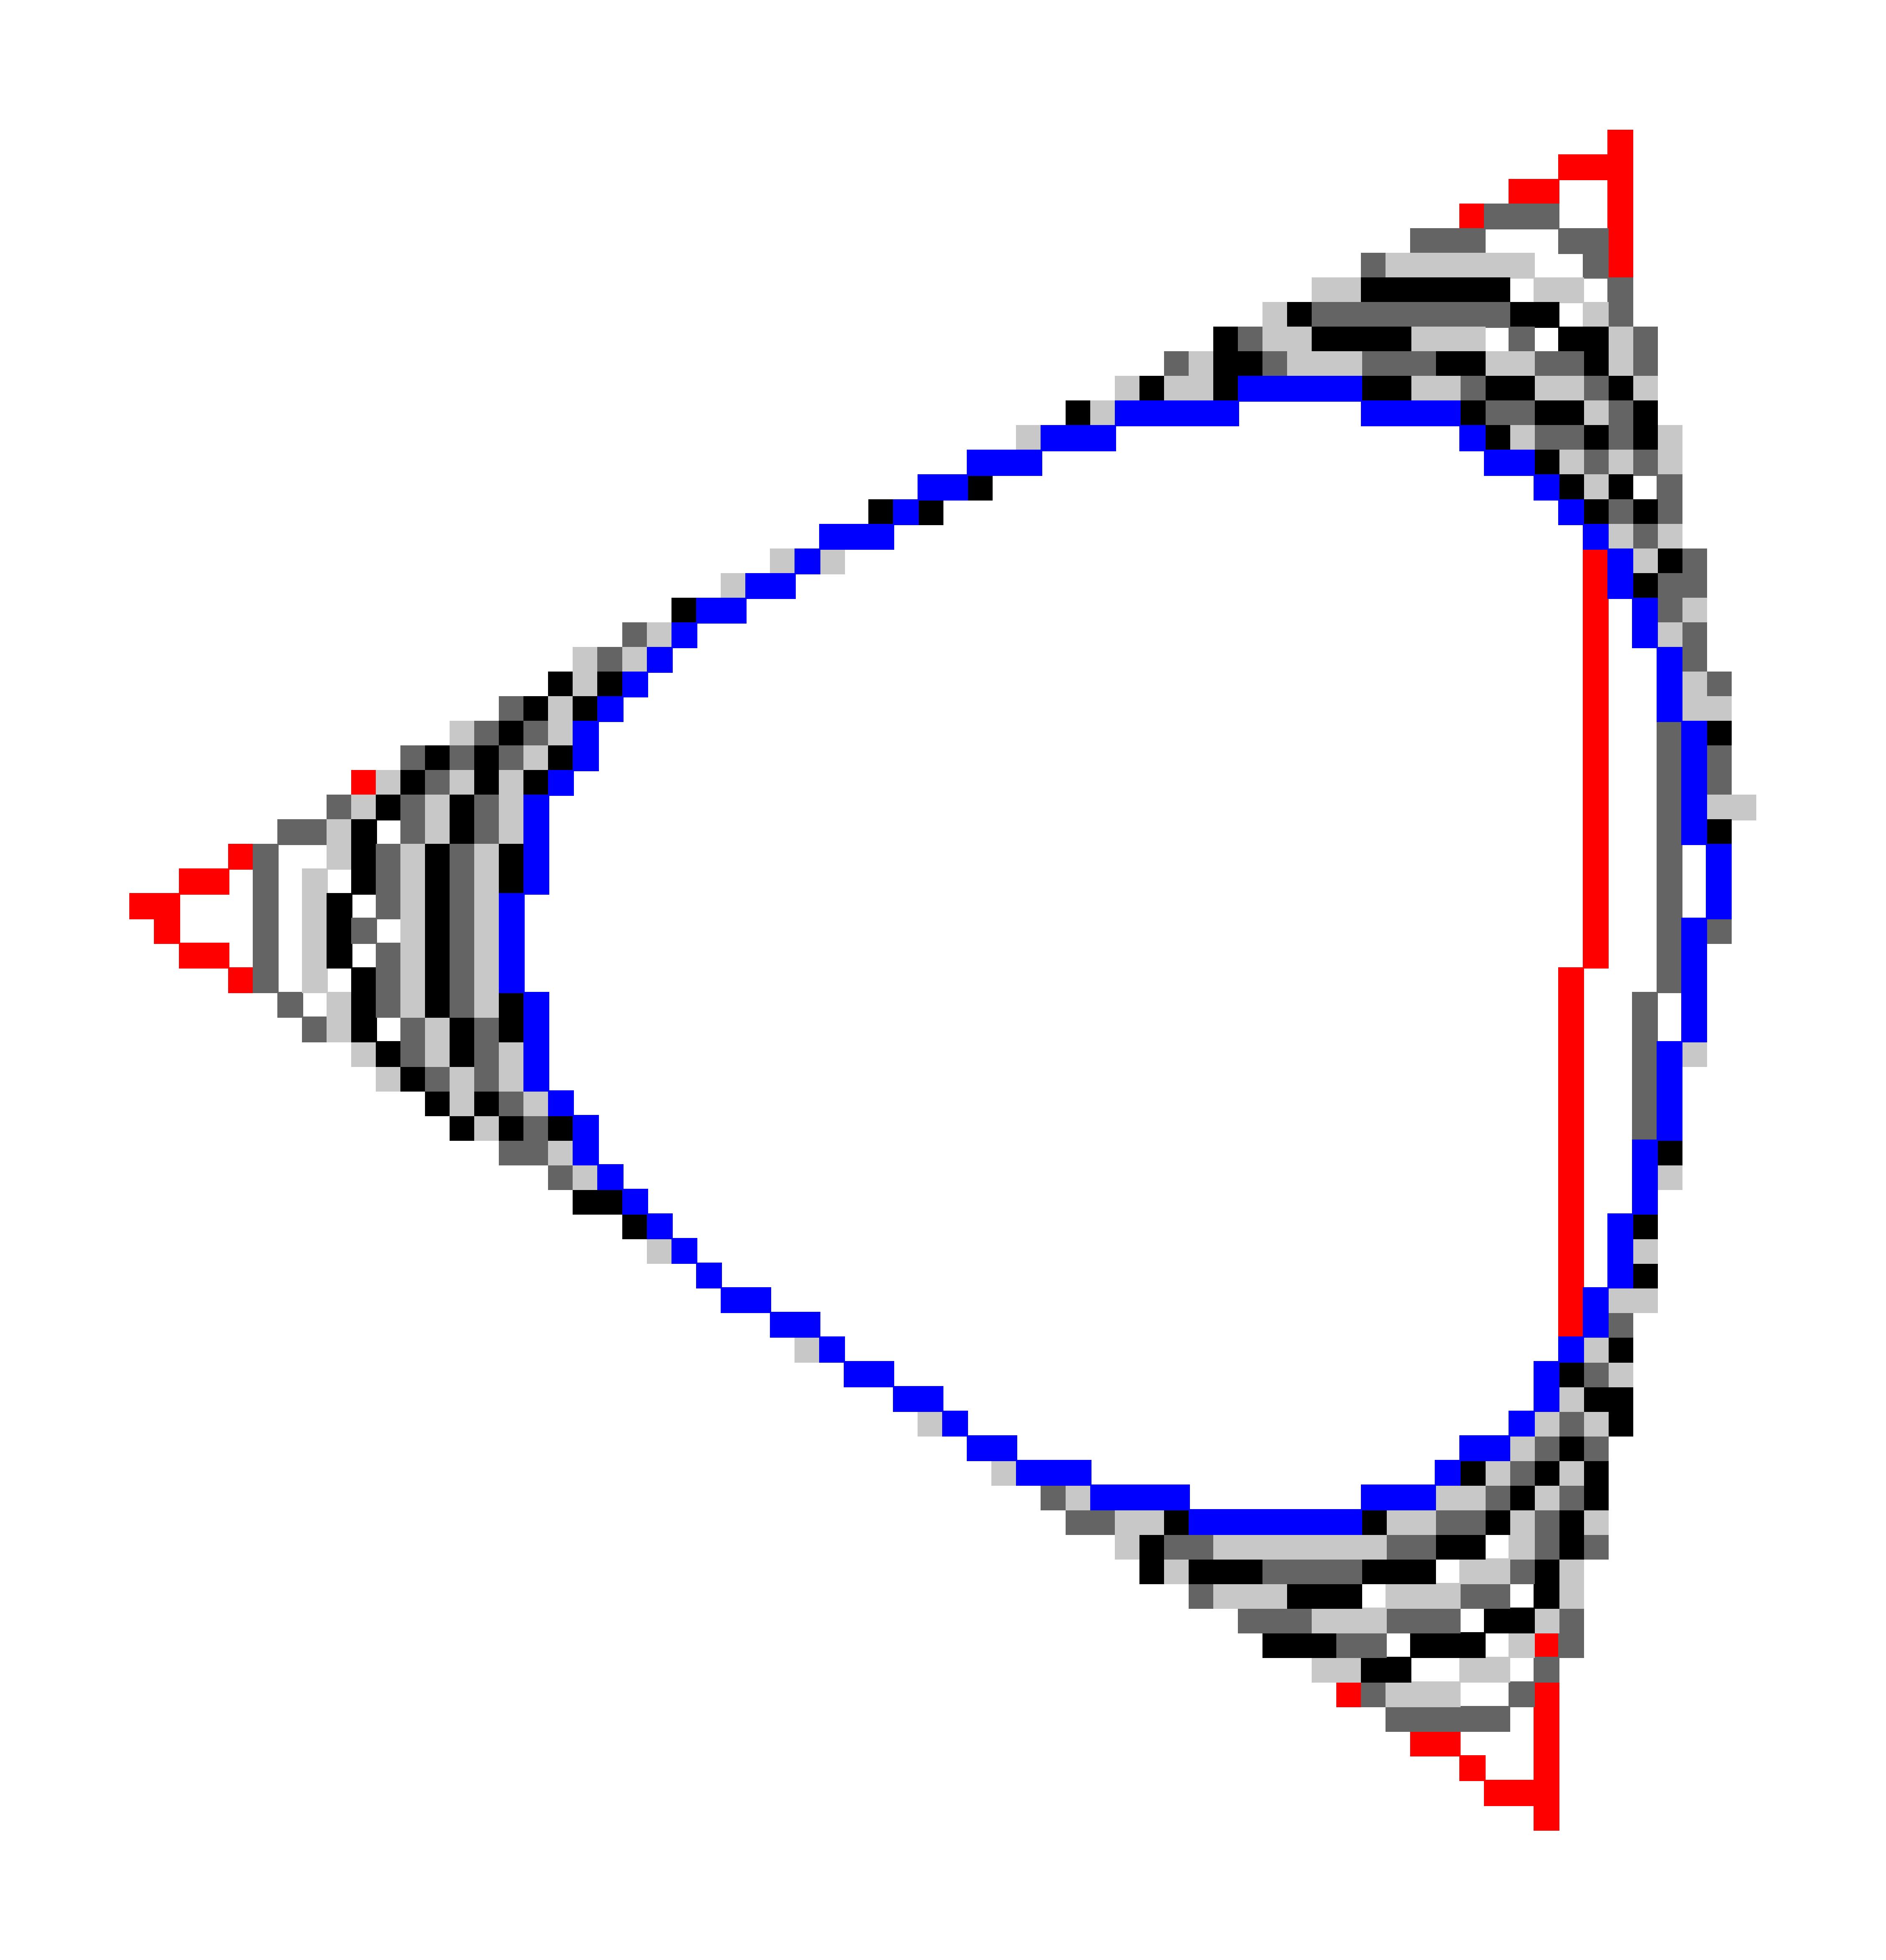
\includegraphics[scale=0.03]{images/Triangle.eps}}%
		\hspace{15pt}
		\subfloat[\label{fig:flow_square}]{%

\includegraphics[scale=0.03]{images/Square.eps}}%		
		\hspace{15pt}
		\subfloat[\label{fig:flow_flower}]{%

\includegraphics[scale=0.025]{images/Flower.eps}}%
		\caption{Digital curvature flow of different shapes. The initial curve is in red and the end curve in blue.}
		\label{fig:digital_flows}	
	\end{figure}


\begin{figure}[!ht]
\center
\begin{tabular}{l|c|c|c|c}
	Energy/Instance & Ball & Triangle & Square & Flower\\
	\hline
	Initial Elastica & 0.156 & 2.55 & 1.81 & 4.196 \\
	Final Elastica & 0.174 & 0.319 & 0.232 & 0.244
\end{tabular}
\caption{Evaluation of digital elastica for start and end objects of the flow.}
\label{tab:digital_glows_elastica_result}
\end{figure}

\subsection{Optimization Method}\label{sec:optimization_method}

	Energy \eqref{eq:corner-detector-opt-exp} is non-submodular and optimizing it is a NP-hard problem, which restrict ourselves to heuristics and approximation algorithms. The QPBO method \cite{kolmogorov07} transforms the original problem in a max-flow/min-cut problem and returns a full optimal labeling for submodular energies. For non-submodular energies the method is guaranteed to return a partial labeling with the property that the set of labeled variables is part of an optimal solution. That property is called partial optimality. 

	In practice, QPBO can left many pixels unlabeled. There exist two extensions of QPBO that tries to overcome this limitation: QPBOI (improve) and QPBOP (probe). The first is an approximation method that is guaranteed to not increase the energy, but we lost the property of partial optimality. The second is an exact method which is reported to label more variables than QPBO. We use QPBOP.
	
\section{Application in Image Segmentation}

The digital curvature flow can be applied as a post-processing step in a image segmentaion framework. We use graph cut \cite{boykov01} as segmentation method and we execute the flow for $n$ iterations. We include the graph cut data attachement term $g$ and standard length penalization $s$ to the flow energy.



\begin{align}			
	\min_{Y} \sum_{y \in Y}{\left( \alpha \cdot s(y) + \gamma \cdot g(y) \right)} + \beta \cdot \sum_{p \in A}{\hat{\kappa}_{r}^2(p)},
	\label{eq:boundary-correction-energy}
\end{align}
	
	where $s(y)=\sum_{\mathcal{N}_4(y)}{ (y-y_k) }^2$.
	


%
% ---- Bibliography ----
%
% BibTeX users should specify bibliography style 'splncs04'.
% References will then be sorted and formatted in the correct style.
%
\bibliographystyle{splncs04}
\bibliography{bibliography}

\end{document}
